\documentclass[10pt]{article}
\usepackage[margin=0.75in]{geometry}
\usepackage{graphicx,booktabs,amsmath,hyperref,mathptmx}
\hypersetup{colorlinks=true,urlcolor=blue}
\title{Factor-base-reduced S3: a checked continuation}
\author{Quadratic-twist study, PR2381}
\date{25 October 2026; reduced-s3-20261025}
\begin{document}
\sloppy
\maketitle
\noindent\textbf{Executed result.} C++ and independent Rust replay98 size-two
cases, 188 main/twist base comparisons and 1,384 target comparisons. There
are 69 joint useful-rank/closure gains and zero joint useful-rank/homogeneous
cutoff gains. This is finite exact algebra; no timing or speedup is claimed.

\section*{Actual example}
Over $\mathrm F_{43}$ use $E:y^2=x^3+x$, its monic twist
$T:Y^2=X^3+4X$, subgroup order 11, generators $(31,18)$ and $(24,26)$.
The existing models are \texttt{icv1-fp6-t0-74779950} and
\texttt{icv1-fp6-t0-c6a8a47c}. The exact bases are $(4,5),(13,19)$
and $(15,9),(17,6)$.
\begin{center}\begin{tabular}{lrrrr}\toprule
First target & Main raw & Main reduced & Twist raw & Twist reduced\\\midrule
Independent useful rows &0&0&2&2\\
Ordered root pairs &0&0&3&3\\
Finite closure degree &6&4&4&2\\
Unit-refutation degree &5&3&---&---\\
Leading-form cutoff &3&2&3&2\\\bottomrule
\end{tabular}\end{center}
The reduced equations are $41xy+39(x+y)+27$ and
$17xy+3(x+y)+41=17(x-15)(y-15)$. The twist degree-two matrix has
rank 3 in 6 columns and 3 independent root evaluations. The main degree-two
matrix has rank 3 with no roots; its first unit occurs at 3, full closure at 4.

\noindent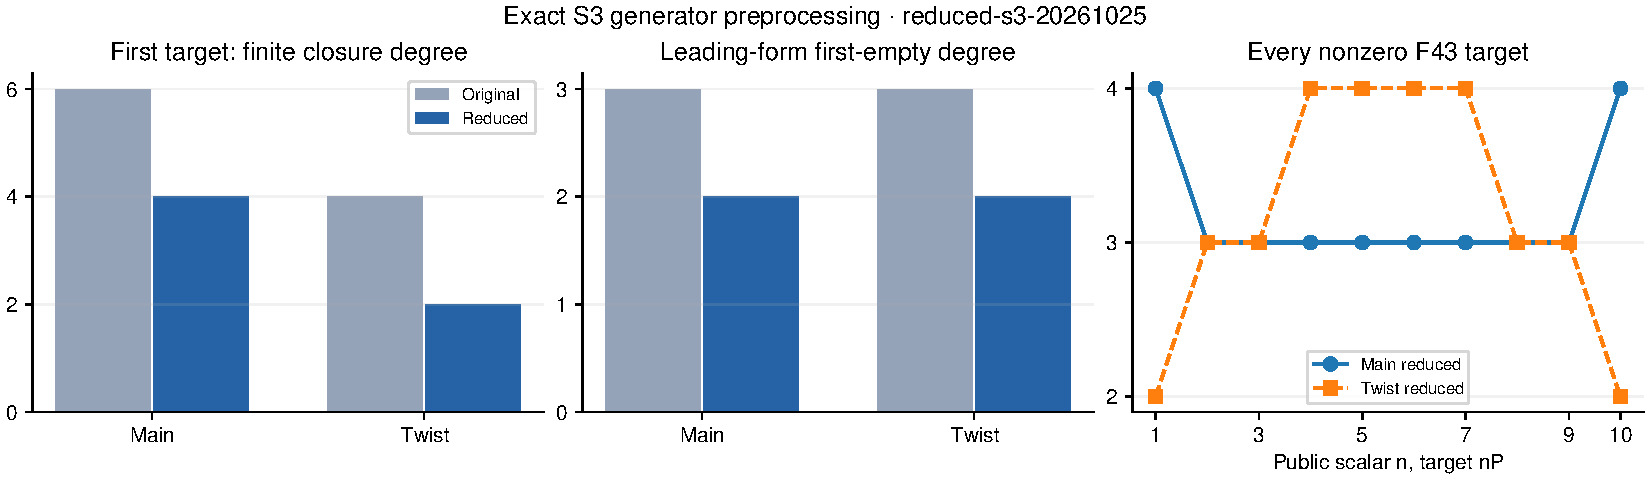
\includegraphics[width=\linewidth]{degrees.pdf}
\noindent\small Recorded native values, including all ten nonzero targets.
The figure source only lays out stored values.\normalsize

\section*{Exact preprocessing and proofs}
For $g_x=x^2-sx+t$ and $g_y=y^2-sy+t$, write
\[
 S_3=(y^2-2zy+z^2)g_x+((s-2z)x+z^2-t)g_y+h,
 \quad h=Axy+B(x+y)+C,
\]
where $A=s^2-4sz-2z^2-2a$,
$B=-st+2zt+sz^2-2az-4b$ and $C=t^2-2tz^2+a^2-4bz$.
The identity is proved over any commutative ring in Lean, together with
equality of the generated ideals and exact equivalence of constrained roots.
The fixture's actual leading ideals normalize to
$\langle xy,x^2,y^2\rangle$ on both arms, with Hilbert vector $(1,2,0,\ldots)$.
Its exact first-empty degree is 2. Because the affine ideal is unchanged,
this input-generator cutoff is not intrinsic regularity of the same ideal
or its saturated homogenization, nor an asserted F4/F5 solving degree.

\newpage
\section*{Scope, independent checks and transfer}
The population consists of all 88 eligible size-two prefixes from the
prior 942-model study plus ten F43 subset policies. All 100 cross-pairings of
the latter are compared. Every nonzero target, actual signed point lift,
coefficient row/rank and homogeneous/affine matrix is independently replayed.
Transported and inverse-transported bases retain identical degree/rank profiles.
The 69 joint closure observations include repeated base-policy comparisons;
they are not 69 independent curves, probabilities or timing trials.

Fifteen new named theorems bring the study to 159 named research theorems and
207 audited declarations across 13 modules. The unmodified scoped gate passes
with zero failing/extra trusted axioms; only propext, Classical.choice and
Quot.sound occur. New declarations include
\texttt{ReducedS3.division\_identity},
\texttt{generated\_ideals\_equal},
\texttt{head\_cutoff\_exact}, and the explicit F43 remainder and head bindings.
The source-bound polynomial certificate \texttt{IDC1h77b3276833a18411}
passes 32+16 native points with false-identity/source controls. Four rehashed
semantic payload controls reject false remainder, degree, rank and omitted case.

The old kernel-checked injective additive map
$\phi(O)=O$, $\phi(x,y)=(41x,11y)$ preserves arbitrary integer scalar relations
and sends the main generator to the chosen twist generator. It is not
defined by a logarithm lookup. The old 11 independent synthetic recoveries
remain historical receipts, not a new recovery run. The generator $(24,26)$
is explicit and is never relabelled as the older generator's EC1 alias.

\section*{Attribution and next experiment}
Preprocessing lowers the leading-form cutoff on both fixture arms; it does
not establish a twist-only homogeneous advantage in this finite population.
Useful yield and finite closure remain target/base dependent. The plot includes
losses. The next lead is adaptive reinsertion of newly found lower-degree rows
and an explicit solver-degree certificate on the same exact inputs. That
follow-up has a draft backlog card and is not executed by this report.
All phase and transfer/recovery costs, a target-matched reference and the
fastest applicable external implementation remain needed before speed claims.

\section*{Reproduction and evidence}
From the repository root, run the versioned protocol's native command:\\
\texttt{bash research/quadratic\_twist\_evidence\_20261021/}\newline
\texttt{run-reduced-s3.sh FRESH\_DIRECTORY}.\\
Sources, compact canonical records and source pins are in
\texttt{native/reduced-s3-20261025}; Lean sources are in
\texttt{lean-reduced}; raw failures, gate receipts, commands and checksums are
in \texttt{validation/reduced-s3-20261025}. Each native command has a 600-second
cap. Python is presentation/metadata only. No prior frozen file or registry,
benchmark or leaderboard row is changed. Shared Conductor still exits 127;
no reservation or substitute coordinator is claimed. Existing CI/review,
integration and mathematical completion gates remain open.
\end{document}
